\documentclass{article} % For LaTeX2e
\usepackage{nips15submit_e,times}
\usepackage{hyperref}
\usepackage{url}
\usepackage{graphicx}
\usepackage{CJKutf8}
\usepackage{hyperref}
%\documentstyle[nips14submit_09,times,art10]{article} % For LaTeX 2.09

\title{Machine Learning Prediction of Chinese Government Censorship on Sina Weibo}


\author{
Alvin Leung \\
Department of Computer Science\\
University of Toronto\\
CSC 2515\\
\texttt{alvinleung94@gmail.com} \\
}

% The \author macro works with any number of authors. There are two commands
% used to separate the names and addresses of multiple authors: \And and \AND.
%
% Using \And between authors leaves it to \LaTeX{} to determine where to break
% the lines. Using \AND forces a linebreak at that point. So, if \LaTeX{}
% puts 3 of 4 authors names on the first line, and the last on the second
% line, try using \AND instead of \And before the third author name.

\newcommand{\fix}{\marginpar{FIX}}
\newcommand{\new}{\marginpar{NEW}}

%\nipsfinalcopy % Uncomment for camera-ready version

\begin{document}
\begin{CJK*}{UTF8}{gbsn}

\maketitle

\begin{abstract}

Chinese social media, in contrast to its Western counterparts, is tightly controlled by the central government. With a database of messages from the Open Weiboscope Data Access initiative, we attempted to solve the supervised classification problem of predicting whether or not a given tweet, or message, on the Sina Weibo microblogging platform will be censored. Using a combination of textual and social features extracted from the message database, an AUC score of 0.95 was achieved using a logistic regression classifier with L2 regularization, with an accuracy of 91\% for censored messages (sensitivity) and 88\% for uncensored messages (specificity). Applying a similar set of features to the problem of predicting the number of days until a censored post is deleted, an average error of 0.9 days was achieved using Support Vector Machine regression.

\end{abstract}

\section{Introduction}
In 2008, China surpassed the United States as the largest group of internet users in the world, and in 2014, Chinese internet users (642 million) account for 22\% of the global number [1]. By 2012, a significant shift in modes of communication had taken place with the rise of social media - an estimated one on every two internet users in China used Sina Weibo, a web microblogging platform akin to Twitter. Usage of email decreased by 10\% in that year, and online forum usage also decreased similarly [2]. Government control of the internet in China is well documented. In particular, politically charged or sensitive statements are prone to be removed without the original poster's consent, through a complex system of router keyword identification as well as a large government employed team of censors who manually read and mark messages for deletion [3]. In addition to deletion, messages posted on forums or blogs can also be altered or only partially removed [4]. Censorship also takes the form of the well-known system of IP and DNS filtering as part of the "Great Firewall", disallowing chinese internet users from accessing foreign websites such as Google, Facebook, Youtube, and Twitter, through careful coordination with ISP's. Much of previous work has focused on this aspect of censorship, with message deletion on starting to be explored in depth using automated methods that do not depend on finding blacklists of filtered words [5] .

\section{Previous Work}

Bammam et al. [5] were one of the first groups to uncover a set of politically sensitive terms whose inclusion leads to anomalously higher rates of deletion, as well as noticing a trend in the location of posting (western provinces tended to have higher censorship rates than the wealthier eastern provinces). [3] and [6] examine the use of homophones by internet users to bypass censorship, and found that 99 \% of homophonic reconstructions of sensitive keywords were clearly intelligible to the average internet user. [7] examined message self-deletion on the Twitter platform, using machine learning classification with textual and social features very much similar to the ones used in this project. 

Important statistical analyses of censorship was performed in [8], where they found that Weibo censorship dynamically changed with the rise in popularity of new topics through multiple layers of filtering. Work by [9] examines the same classification problem, but uses a much smaller dataset between June and August of 2012, focusing on connecting censored messages with a timeline of political events. As well, it was found that [9] inadvertently included the "deletion" field of the dataset, and the very good results obtained is likely due to training on data with a field that contains the answer to the classification problem. [10] attempts to build an automatic detector of censorship by modelling communication as a graph and using topological features to train a classifier. 

\section{Methods}
The database or messages was constructed using a random sampling approach detailed in [11]. The pattern of usage was analyzed for 30 000 Weibo accounts and messages were randomly pulled from users' timelines over a 12 month period, and they were periodically automatically checked for deletion. The difference between a user deleting her/her own post and the government deleting the post is documented as well, because self deletion garners a different error message than censored deletion when an attempt is made to access a deleted post through the Weibo API. In addition to sampling the messages, information about the user including age, gender, province, and post history were also gathered. Of the 226841122 sampled messages, 86083 were found to have been deleted through censorship. This leads to an estimate of censorship that is much lower than previous estimates. The problem of severe class size imbalance between censored and uncensored messages was solved by random sampling of uncensored messages (greatly undersampling), while retaining all the censored messages. Features were selected through a forward selection approach, whereby features that improved classification performance were added to the feature list, whereas features that decreased performance were pruned. Recursive feature elimination was also attempted, but yielded poorer results than manual forward selection.

\subsection{Textual Features}
Textual features were extracted from the weibo message body by first parsing strings of Chinese text into the constituent words, and then considering a subset of all unique words used in all messages. Text parsing was done using the ICTCLAS lexical analyzer [12] developed at the Chinese Academy of Sciences. This method was chosen because it is open source and because of its performance on Chinese text segmentation competitions. ICTCLAS text segmentation is based on a Hidden Markov Model approach and includes not only atomic segmentation but recursive unknown word recognition and POS (parts of speech) tagging. The ICTCLAS algorithm can be augmented through the use of custom libraries to expand its base dictionary in order to improve segmentation. Here, we utilized several custom word lists downloaded from the Sogou Pinyin word list database, and the .scel file format was parsed using another open source library [13]. These lists included words in three categories: popular words used in internet slang, names of geographic locations in China, and political terms and titles. The choice of these lists was heuristic based on the nature of the problem. \\

Having parsed all of the messages in the censored messages set and the uncensored messages set, two metrics were employed for feature selection: word frequency and mutual information. For word frequency, two dictionaries were written - one with the count of all 53916 words used in censored messages, and one with counts for all 518303 uncensored messages. We found many words used in the censored messages but never found in uncensored messages (even though the sample size for uncensored is 2 orders of magnitude larger). Disregarding rare words that are used less than ten times in total, this indicates some degree of absolute keyword filtering for the words in this list that are left. \\ 

To calculate the correlation between each word term $x_{i}$ and the censorship class (either 1 for censored or 0 for uncensored), we used the common NLP mutual information metric:

\begin{center}
$\sum_{x_{i}\in{0,1}}\sum_{y\in{0,1}}p(x_{i},y)log_{2}\frac{p(x_{i},y)}{p(x_{i})p(y)}$
\end{center}

Where $x_{i}$ refers to the ith word out of all words used in all messages, and the probabilities $p(x_{i},y) = p(x_{i}|y)p(y)$, $p(x_{i})$, and $p(y)$ were calculated from their maximum likelihood estimates based on their respective counts in data - $p(x_{i}|y)$ was estimated from the number of messages containing the word $x_{i}$ and had class label y, $p(x_{i})$ was estimated from the number of messages containing $x_{i}$ divided by the number of all words, and $p(y)$ was the proportion of messages with that class label.  

\begin{figure}[!htb]
	\begin{center}
		    \begin{tabular}{ | l | l | l | l | l | l |}
		    \hline
		    人民 & 0.0025301394893 & 地址 & 0.0007382394232& 媒体 & 0.0005251610648 \\ \hline
		    中国 & 0.0016069369411 & 什邡 & 0.0007102348984 & 求证 & 0.0005167170327\\ \hline
		    书记 & 0.0013981448299 & 爱   &0.0007067656087 & 表哥& 0.0005039648846\\ \hline
		  [话筒] & 0.0011768666274 & 腐   & 0.0006746895380& 辟谣& 0.0004958811960\\\hline
		   	政府 & 0.0011183962839 & 反   & 0.0006389173540& 公开 & 0.0004899889207\\\hline
		    官员 & 0.0010661401811 & 民主 & 0.0006181865769 & 干部 & 0.0004830381873\\\hline
		    党 & 0.0009633692457 & 表叔 & 0.0006088447928 & 马碧 & 0.0004720284947\\\hline
		    重庆 & 0.0009525769341 & 网络 & 0.0005862150697 & 习 & 0.0004633658489\\\hline
		    删 & 0.0008791662092 & 说 & 0.0005837134953 & 权力 & 0.0004537628632\\\hline
		    财产 & 0.0008714853341 & 文革 & 0.0005680067882 & [爱你] & 0.0004524005934\\\hline
		    国家 & 0.0008586612231 & 公民 & 0.0005496450495 & 老百姓 & 0.0004425673047\\\hline
		    领导 & 0.0008217471100 & 座 & 0.0005444427729 & 中央 & 0.0004380197011\\\hline
		    斯巴达 & 0.0007674227947 & 百姓 & 0.0005382390613 & 官& 0.0004376716948\\\hline
		    政治 & 0.0007588748087 & 改革 & 0.0005300021423 & 贪官 & 0.0004364276704\\\hline
		    民 & 0.0007548637623 & 历史 & 0.0005278915392 & 喜欢 & 0.0004347288152\\\hline
		    \end{tabular}
	\end{center}
\caption{A table showing the top 45 words that have the highest mutual information with the random variable Y representing the censorship outcome.}
\vspace{-10pt}
\end{figure}
The mutual information metric yielded a ranked list of features that were useful for distinguishing censored and uncensored messages, and the presence or absence of the top MI words were used as inputs for our classification algorithm. We can see from the top words that many of them are politically motivated, including "the people", "officials", "china", "government", "politics", "cultural revolution", etc. In addition, many terms were in fact the actual names of political officials whose criticism or even mention is presumably disallowed, such as 马碧, a party secretary general of the standing committee of a city in Guangdong province. It is interesting to note that high on the list not only included extracted words correlating with censored messages but also those correlating with uncensored messages, such as 爱你, which presumably would not usually be part of censored messages. 

\subsection{Other Features}
In addition to classifying the messages using textual features, we also added social features that made a significant impact on the classification results. In particular, whether the tweet was accompanied by an image or not, the gender of the user who posted the message, the province in which the user lives, and whether or not the message was retweeted (reposted from another person's wall) all contributed to improving the classification. Censored messages tended to be posted by male users, did not include images, and were more likely to be retweeted than uncensored messages, possibly because retweeting a message increases its exposure and thus chance of deletion. Another particularly informative feature was the count of how many messages posted by the user who posted a message have been previously censored. The rationale behind this is that people who tend to actively engage in political discussions will be repeatedly censored, whereas people who generally do not post about taboo topics will not be censored. It was found that account verification and the date or month of posting had no impact on classification results. 

\begin{figure}[!htb]
	\begin{center}
		    \begin{tabular}{ | l | l | l |}
		    \hline
		    & Censored & Uncensored \\\hline
		    Image & 9.94\%& 25.91\% \\ \hline
		   	Retweeted & 82.97\% & 63.96\% \\ \hline
		  	Male & 84.93\% & 45.98\% \\\hline
		   	Account Verified & 34.05\% & 25.78\%\\\hline

		    \end{tabular}
	\end{center}
\caption{A table showing various social features and their percentages in the censored and uncensored samples respectively.}
\vspace{-10pt}
\end{figure}

\begin{figure}[!htb]
	\begin{center}
	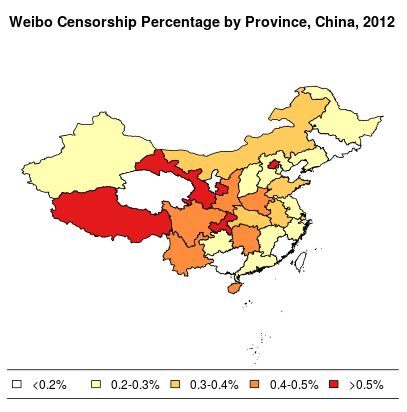
\includegraphics[width=0.65\textwidth, height = 0.4\textheight]{./pynlpir/chinaplot}
	\end{center}
\caption{Map of China showing extent of censorship among all sampled messages originating from that province in 2012.}
\vspace{-10pt}
\end{figure}

\section{Results}

The machine learning predictions generated using the robust scikit-learn package for python, and visualizations were done using matplotlib. We used several different classification algorithms to train the data with and evaluate the results - logistic regression with l1 and l2 regularization, logistic regression with stochastic gradient descent as the optimization algorithm, k-nearest-neighbors with a variable k, support vector machine classification, and naive (bernoulli) bayes, which has been shown to yield good results in text classification applications. The proportion of training and testing examples was determined to be 4/5 training and 1/5 testing data. 

Many parameters had to be fine tuned to optimize classification performance. Although a larger data set leads to better performance because it can provide a larger number of training samples, the large class imbalance means that there is a point where adding more uncensored training examples does not improve and actually decreases performance. A key parameter to vary was the class weights, which were used in logistic regression in order to balance the class sample sizes. An optimal (best AUC score) class weight ratio of 0.3 for uncensored data and 0.7 for censored data was found for our particular sample size (as described in the methods). Also, it was important to  determine the optimal number of feature words (from the top mutual information list) used as input features in order to try to avoid overfitting the training data. The number of feature words was also reduced for practical runtime considerations, as the large amount of batch training consumed all of the system's resources, leading to memory errors. 2500 words struck a balance between runtime and performance - over 5000 gave memory errors, and less than 2000 gave markedly decreased performance. This was also the motivation behind using Stochastic Gradient Descent for logistic regression as one of the classification algorithms, because SGD allows for online (or mini-batch) learning. However, SGD is random by nature and produces sub-optimal results. Of course, the model parameters such as the dropoff tolerance and the regularization constant also needed to be determined, and this was done using a grid search cross validation method of optimizing the combinations of a varied number of parameters.


\begin{figure}[!htb]
	\begin{center}
		    \begin{tabular}{ | l | l | l | l | l | l |}
		    \hline
		    斯巴达 & 4.2922599219733 & 两会 & 1.5553773382597& 薄 & 1.2666734418383 \\ \hline
		    习 & 2.7551977907267& 薄熙来 & 1.5236911442546 & 死者 & 1.2637686300884\\ \hline
		   李彦宏 & 1.8972207368863 & 元芳 & 1.5228466347735 & 传言 & 1.2483999482497\\ \hline
		  莫言 & 1.8702632585227 & 入党 & 1.4937699447154& 反日 & 1.2373959792604\\\hline
		   	陈光诚 & 1.8279651246137& 总理 & 1.4645516378991& 毛主席 & 1.2331771751226\\\hline
		    十八大 & 1.7902065984958 & 搜索 & 1.4455616148594 & 编译 & 1.2312446523401\\\hline
		   求证 & 1.7289662468372 & 删 & 1.4345862145740 & 暴徒 & 1.2282004880148\\\hline
		   水面 & 1.7223489264977& 书记 & 1.4235296365612 & 雷锋 & 1.2268196641473\\\hline
		    12秒 & 1.7182631898935 & 洗脑 & 1.3942328420659 & 二炮 & 1.2026844314020\\\hline
		   什邡 & 1.7052428141964 & 捐你妹 & 1.3937658526473 & 长江 & 1.2002928948723\\\hline
		   习近平 & 1.6963815578815 & 自焚 & 1.3271996789806 & 干部 & 1.1912406812331\\\hline
		    [国旗] & 1.6824662271172 & 彭丽媛 & 1.3197186503643& 财产 & 1.1907213082163\\\hline
		   翻墙 & 1.6796898494824& 政治局 & 1.3039797742135 & 新闻联播 & 1.1858537632922\\\hline
		    启东 & 1.6659106393678 & [走你] & 1.2966450251884& 民 & 1.1853948050426\\\hline
		    喜迎 & 1.5722041194372 & 王立军 & 1.2853849215898 & PX & 1.1830316768194\\\hline
		    \end{tabular}
	\end{center}
\caption{A table showing the top 45 features with the highest parameter coefficient values - all of these happen to be words, although other social features are also on this list.}
\vspace{-10pt}
\end{figure}

Table 3 above shows features with highest weights in L2 regularized logistic regression. It is remarkable that these features seem obviously important and related to the censorship problem. The first and sixth term both refer to the Communist Party Congress, Mo Yan is one of the most famous authors of modern China and his works are often banned, 陈光诚 is a famous civil rights activist, and even 习近平 appears in this list.  Three major protest events are represented: 什邡 was the site of a massive protest because of the construction of a copper refinery plant, 启东 was the site of another environmental protest, this time over the construction of a waste-water pipeline that would have dumped massive amounts of industrial waste into the sea, and in 2012 there were also two rounds of civil unrest related to sovereignty over the Senkaku Islands, which stirred up a lot of anti-Japanese sentiment.  


\begin{figure}[!htb]
	\begin{center}
		    \begin{tabular}{ |l | l | l | l |}
		    \hline
		    & AUC & Sensitivity & Specificity \\\hline
		    Logistic Regression (L2 Regularization) & 0.94784 & 0.90500 & 0.87685 \\ \hline
		    Logistic Regression (L1 Regularization) & 0.94655 & 0.90246 & 0.87647 \\ \hline
		  	Logistic Regression (L2 Regularization, SGD) & 0.94527 & 0.85206 & 0.91865 \\\hline
		   	Naive Bayes & 0.94019 & 0.83086 & 0.91765\\\hline
		   	K-Nearest-Neighbors & 0.89644 & 0.82912 & 0.92088\\\hline
		    \end{tabular}
	\end{center}
\caption{A table showing the classification performance of various machine learning algorithms.}
\vspace{-10pt}
\end{figure}

L2 regularized logistic regression gave the best performance out of all of the classification algorithms, but the performance was similar across all the models. The features selected did not overfit the data, and we achieved good performance with Naive Bayes and KNN as well. Support Vector Machine classification could not be completed due to memory errors. We postulate that support vector machine or other maximum margin classifiers would give even better performance than simple regularized logistic regression, because the data appears to be mostly linearly separable. The feature vectors, being an array of mostly 1's and 0's representing the presence or absence of a word in the message, formed a very sparse and high dimensional feature space, which is probably why KNN performance was not as good as logistic regression. 

\begin{figure}[!htb]
	\begin{center}
	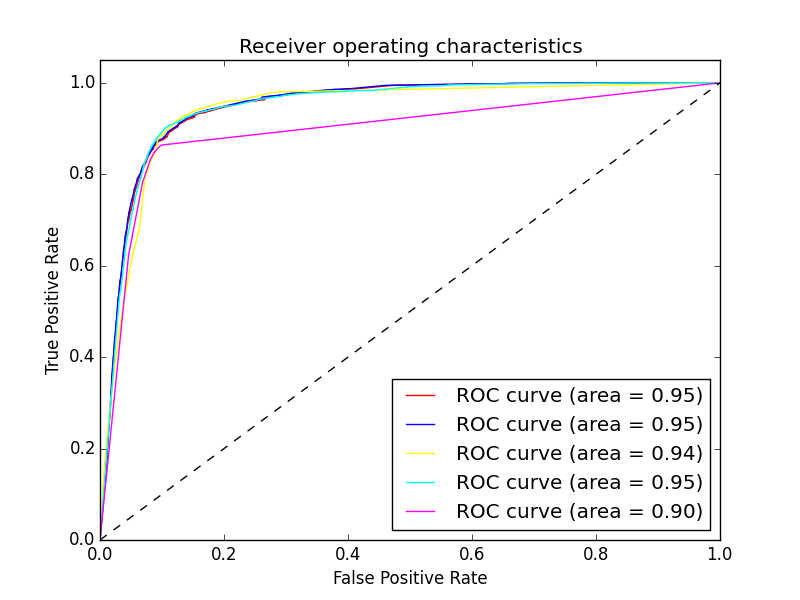
\includegraphics[width=0.82\textwidth, height = 0.4\textheight]{ROC_Curve}
	\end{center}
\caption{Receiver Operating Characteristic curves for the various classification algorithms. L1 logistic regression - red, L2 logistic regression - blue, naive bayes - yellow, stochastic gradient descent - cyan, KNN - magenta}
\vspace{-10pt}
\end{figure}

The problem of predicting the time (in days) from a message is posted until it is censored was also attempted using simple regularized linear regression and support vector machine regression. The same features that were used in classification were applied here, although it was determined that a feature word set size of about 100 was optimal, as opposed to a much higher number for the classification task. The average absolute value error metric used to evaluate the results of regression needs to be improved, as large amount of 0-valued deletion times in addition to small amounts of large valued deletion times means that the algorithms are trained to give small deletion times, at minimal expense of the large valued deletion times, which are equally valuable to determine. 

\begin{figure}[!htb]
	\begin{center}
		    \begin{tabular}{ |l | l | l |}
		    \hline
		    & Average Abs. Value of Error & Standard Deviation of Error \\\hline
		    Linear Ridge Regression & 2.3565 & 2.3200 \\\hline
		    Support Vector Machine & 0.9983 & 2.6253 \\ \hline
		    \end{tabular}
	\end{center}
\caption{A table showing the regression performance for predicting deletion time.}
\vspace{-10pt}
\end{figure}

\section{Conclusions and Future Work}
In this project, we achieved a decent result for classifying an arbitrary posted message as censored or uncensored by the Chinese government. With similar techniques, we can develop systems to warn netizens that their posts are likely to be deleted, or simply to raise awareness about internet censorship and make available posts that are not meant to be seen. This approach, in contrast to earlier approaches of figuring out authoritative blacklists and words with high likelihood of being filtered or trying to reverse engineer the flow of packets through the network, can be generalized much more easily to arbitrary censorship systems, and new "blacklists" can be dynamically generated with each new training example. With a regression algorithm that can tell us the likely time a post will be censored, we can potentially circumvent censorship by automatically reposting messages before their destined deletion time.  

In addition to the other informative features included in the message database, one other metric of sentiment analysis was attempted. A list of positive and negative sentiment words were searched through for each message and the ratio of positive and negative sentiment words present in the message with all sentiment words was added to the feature list. Surprisingly, this also had little impact on the results. The sentiment metric was likely too broad and unrealistic to be used, and future work will likely benefit from an improved measurement of the message sentiment. 

Since 2012, China has made significant investments into Internet filtering and censorship technology, including but not limited to big data approaches to deleting politically sensitive messages on social media platforms. As such, it will become increasingly difficult to be able to track censored messages via calls to a platform's API (as was done in compiling the dataset used in this project) because much of the deletion will occur automatically, before any public access. Future work in this field must leverage the fact that censorship is increasingly done automatically using a combination of big data analytics, natural language processing and sentiment analysis, as opposed to by a team of manual censors. 

\section{References}
All the code for this project can be found at \url{https://github.com/coolestcat/weibo-censorship-project}

[1] "Internet Users Live Stats." Number of (2015). Web. 14 Dec. 2015.

[2] China Internet Network Information Center (2012) "30th statistical report on Internet development in China." Beijing, China: China Internet Network Information Center

[3] King-wa Fu; Chung-hong Chan; Chau, M., "Assessing Censorship on Microblogs in China: Discriminatory Keyword Analysis and the Real-Name Registration Policy," (2003) in Internet Computing, IEEE , vol.17, no.3, pp.42-50 doi: 10.1109/MIC.2013.28

[4] Mackinnon, Rebecca. "China’s Censorship 2.0: How companies censor bloggers." First Monday, [S.l.], jan. (2009) ISSN 13960466. Date accessed: 13 Dec. 2015. doi:10.5210/fm.v14i2.2378.

[5] Bammam, David; O'Connor, Brendan; Smith, Noah. "Censorship and deletion practices in Chinese social media." (2012) First Monday, [S.l.], mar. ISSN 13960466. Date accessed: 13 Dec. 2015. doi:10.5210/fm.v17i3.3943.

[6] Hiruncharoenvate, C., Lin, Z. and Gilbert, E. (2015). Algorithmically Bypassing Censorship on Sina Weibo with Nondeterministic Homophone Substitutions.. In M. Cha, C. Mascolo and C. Sandvig (eds.), ICWSM (p./pp. 150-158), : AAAI Press. ISBN: 978-1-57735-733-9 

[7] Petrovic, S., Osborne, M., Lavrenko, V. (2013). I Wish I Didn't Say That! Analyzing and Predicting Deleted Messages in Twitter. arXiv:1305.3107

[8] Zhu, Tao, et al. "Tracking and quantifying censorship on a Chinese microblogging site." arXiv preprint arXiv:1211.6166 (2012).

[9] Li, J.(2015). Predicting Large-Scale Internet Censorship - A Machine Learning Approach. Retrieved from http://libra.virginia.edu/catalog/libra-oa:9531

[10] Morrison, Donn. "Toward automatic censorship detection in microblogs." Trends and Applications in Knowledge Discovery and Data Mining. Springer International Publishing, 2014. 572-583.

[11] Fu, K. and Chau, M. (2013). Reality Check for the Chinese Microblog Space: A Random Sampling Approach. PLoS ONE, 8(3), p.e58356.

[12] Zhang, H., Yu, H., Xiong, D. and Liu, Q. (2003). HHMM-based Chinese lexical analyzer ICTCLAS. Proceedings of the second SIGHAN workshop on Chinese language processing.

[13] Guo, HW. (2015) Scel2Txt. Retrieved from https://github.com/haowg/Scel2Txt

\clearpage\end{CJK*}
\end{document}